\chapter{Introduction}\label{introchapter}
The auditory system is among the most ubiquitious of sensory systems as evidenced by the 
development of numerous strategies for the detection and processing of auditory stimuli
across several species. The processing of sound stimuli is fairly fast and in comparison
to light stimuli, sound has two main properties - it is omnidirectional and due to
its large wavelength, it isn't blocked by small objects. For instance we can hear objects
behind us or behind obstacles whereas the same isn't true for visual stimuli. These properties 
give the animal the obvious advantage of being able to react to approaching dangers that
aren't yet visible. In order to fully utilize the sound stimuli, it is therefore essential
that an animal is able to assess the direction or, to use the technical term, \textit{localize} a sound source.

Before we discuss the various sound localization methods observed in nature, we first
go through the fundamental steps involved in auditory perception. First, an object generates
an auditory stimulus which in general can be very complex. This stimulus then propagates
through a given medium (e.g. air, water) and excites the primary receiver(s) of the animal. In most
terrestrial vertebrates, these take the form of \textit{tympani} or eardrums - a pair of thin vibrating
membranes which are a component of the mechanical part of the auditory system.
Depending on the species, there may be an apparatus that focuses and amplifies the sound waves. In
humans for example, this function performed by the external ears or pinnae. 
The vibrations are then transmitted by means of a set of bony or cartilaginous elements and
converted into electrochemical signals that will be processed neuronally; see Sec. \ref{mechanicalprocessing}.

The neuronal processing system consists of building blocks called \textit{neurons} which are
connected to eachother through \textit{synapses}. The entire system is referred to as a 
\textit{neuronal net}. The neuronal computation gives rise to a representations of the stimuli
known as \textit{neuronal maps}. Each neuron of the map represents a specific property, e.g.
the position in space or the frequency of the stimulus and neighbouring neurons respond to
similar sensory inputs. Neuronal maps serve to reconstruct stimuli as optimally as possible
within the limits of processing. The precise calibration of the
synapses required for stimulus reconstruction is a result of experience-based learning
processes that take into account inputs from all available sensory systems.

The primary focus of this thesis is the mechanical processing that is responsible for the
sound localization ability of certain terrestrial vertebrates. Specifically, we are interested
animals that have their eardrums connected through a large mouth cavity and the emergence of
 directionality in the response of such systems.

\section{Mechanical Processing of Auditory Stimuli}\label{mechanicalprocessing}

\begin{figure}
 %\centering
 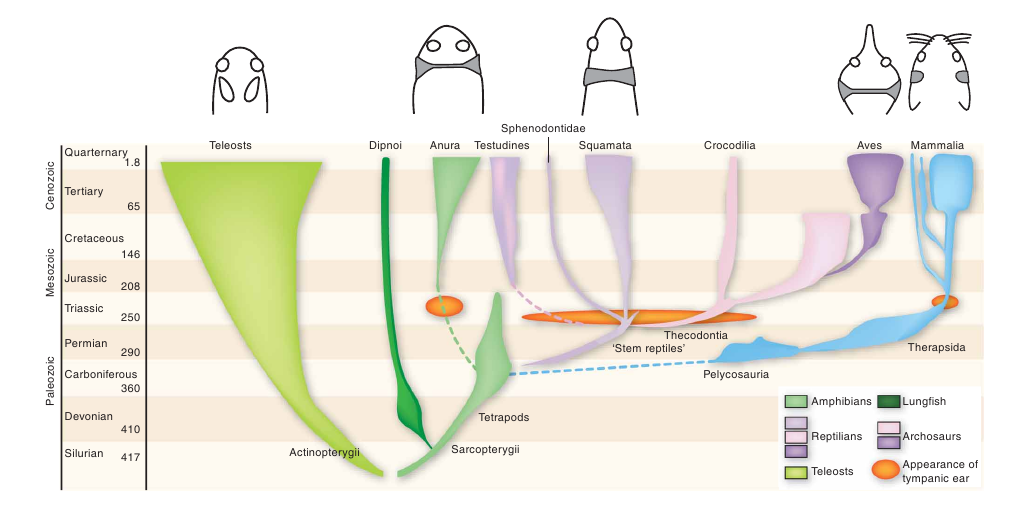
\includegraphics[width=1.0\linewidth]{Diagrams/vertebrateearevolution.png}
 \caption[Vertebrate Ear Evolution]{Figure due to Schnupp and Carr \cite{schnuppcarr}.}
 \label{vertebrateearevolution}
\end{figure}